\chapter{Implementación}

\section{Diseño del Sofware}

\begin{figure}[!h]
    \centering
    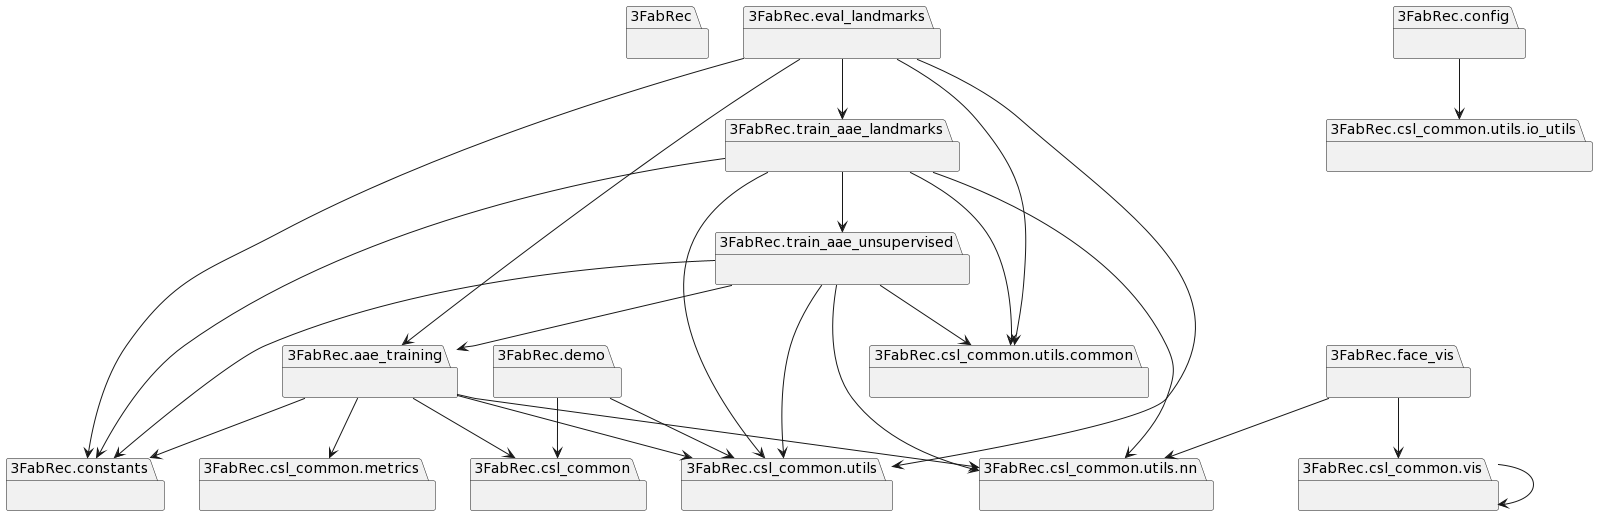
\includegraphics[width=0.9\textwidth]{img/diagrama_paquetes_1.png}
    \caption{Diagrama de paquetes del proyecto.}
    \label{fig:Diagrama_paquetes}
\end{figure}


\begin{figure}[!h]
    \centering
    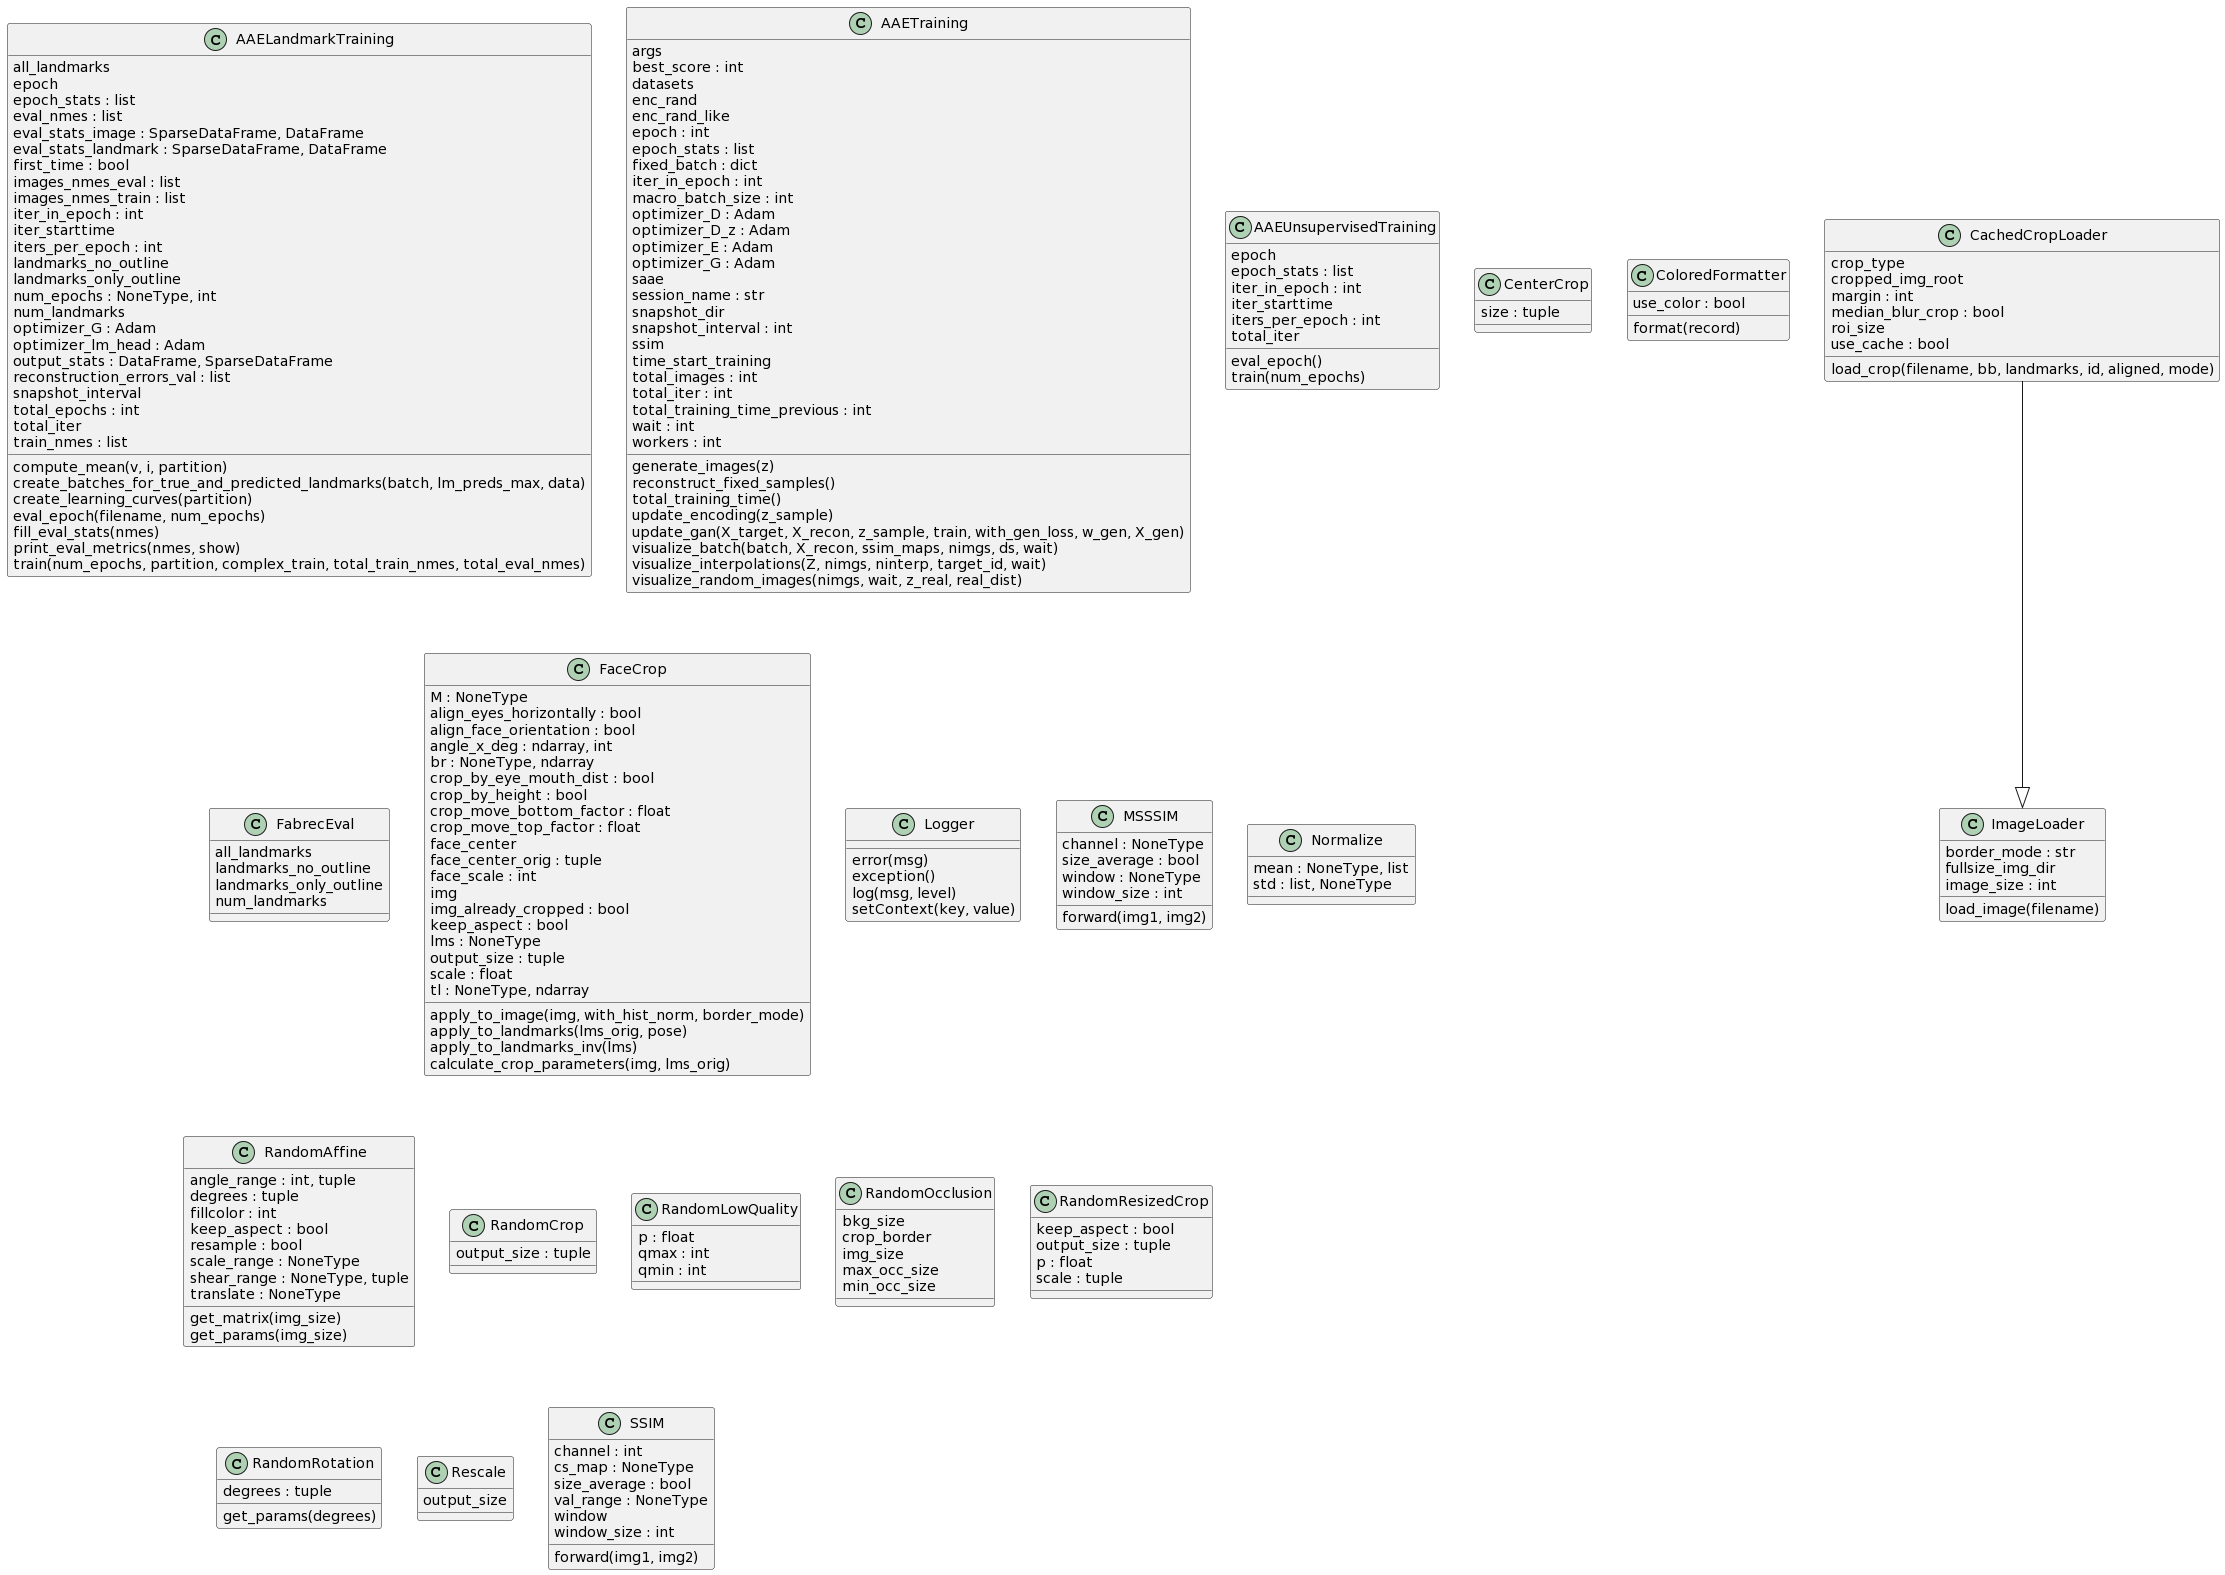
\includegraphics[width=0.9\textwidth]{img/diagrama_clases.png}
    \caption{Diagrama de clases con las principales clases del proyecto.}
    \label{fig:Diagrama_clases}
\end{figure}

\section{Entorno de ejecución}
\noindent Las ejecuciones se han realizado todas en un ordenador portátil \textit{HP Pavilion} con las siguientes características: 

\begin{itemize}
    \item Ubuntu $20.04.5$ LTS $64$ bits.
    \item $8$ GB de RAM
    \item $8$ x Intel® Core™ i$5$-$8300$H CPU @ $2.30$GHz
    \item GPU NVIDIA GeForce GTX $1050$ Mobile
\end{itemize}

\medskip

\noindent Por otro lado, las versiones del software empleado son: 

\begin{itemize}
    \item Python 3.6.13
    \item CUDA 10.1
    \item PyTorch 1.1.0
    \item Numpy 1.17.4
    \item Pandas 0.23.3
    \item Matplotlib 3.3.4
\end{itemize}


\endinput
%------------------------------------------------------------------------------------
% FIN DEL CAPÍTULO. 
%------------------------------------------------------------------------------------

